% Chapter Template

\chapter{Introduction} % Main chapter title

\label{Chapter1} % Change X to a consecutive number; for referencing this chapter elsewhere, use \ref{ChapterX}

%----------------------------------------------------------------------------------------
%	SECTION 1
%----------------------------------------------------------------------------------------

\section{Motivations and problem statement}

In recent years, the concept of well-being has been the subject of increasing interests for governments, councils, policy makers and researchers, though research on the subject has been happening since the 1970s.
An interesting recent development is a report into well-being in Danish cities by (\cite {OECD16}) which highlights how well-being tools have become an important tool to identify the needs of citizens and the domains where demand for progress is greatest. 

This idea of well-being is often defined using a set of indicators relating to a particular place. There is no universally agreed definition of exactly which factors are the best measures of well-being, however, various indexes and studies show a great deal of commonality on the types of measures that are important to the well-being of citizens.

What is less clear is whether, and how, these indicators affect the real estate values in a specific city. For example, The Greater London Authority created a set of well-being indicators and used them to create a map of well-being by London Ward in 2014 (\cite{GLA14}), however, this was not linked back to real estate values.
In one study looking at linkages between house prices and mental wellbeing, (\cite {AR13}), points out that when people can move freely, each person will maximize wellbeing by moving to areas that best satisfy their preferences; this results in zero correlation between area characteristics (or house prices) and wellbeing. But if people think they are paying too much for poor quality or too little for high quality, we would observe a positive relationship between area characteristics and wellbeing. The study found a positive correlation between house prices and mental wellbeing.

Another hypothesis found in the Economics literature is that real estate values are the drivers of the well-being indicators, happier people are better at generating wealth (\cite {LKD05}), which leaves open the possibility that areas with high well-being provide a flow of people migrating to places with higher real estate values. From the point of view of Data Science it would be interesting to consider the real estate values in bandings such as quintiles as well-being indicators may have a very different relationship with the top 20 percent of areas by real estate value than with areas in the lower four quintiles.

Work on urban scaling (\cite {BLSW10}) suggests that different types of well-being indicators may have different relationships with real estate values due to the non-linear nature of agglomeration. Bettencourt et al. argues that city indicators are governed by power laws rather than linear per-capita indicators. Social factors tend to be superlinear whereas material infrastructure tends to be sublinear at best. There may therefore be some level of divergence between different well-being factors.
This project focuses on the city of London and tries to determine which well-being indicators show a relationship with real-estate values. The findings will be displayed in the form of an interactive map.

This project sets out to create a set of well-being indicators for each administrative ward in London and will attempt to model median house prices based on these indicators.


%----------------------------------------------------------------------------------------
%	SECTION 2
%----------------------------------------------------------------------------------------

\section{Project trailer}

\begin{figure}[H]
\centering
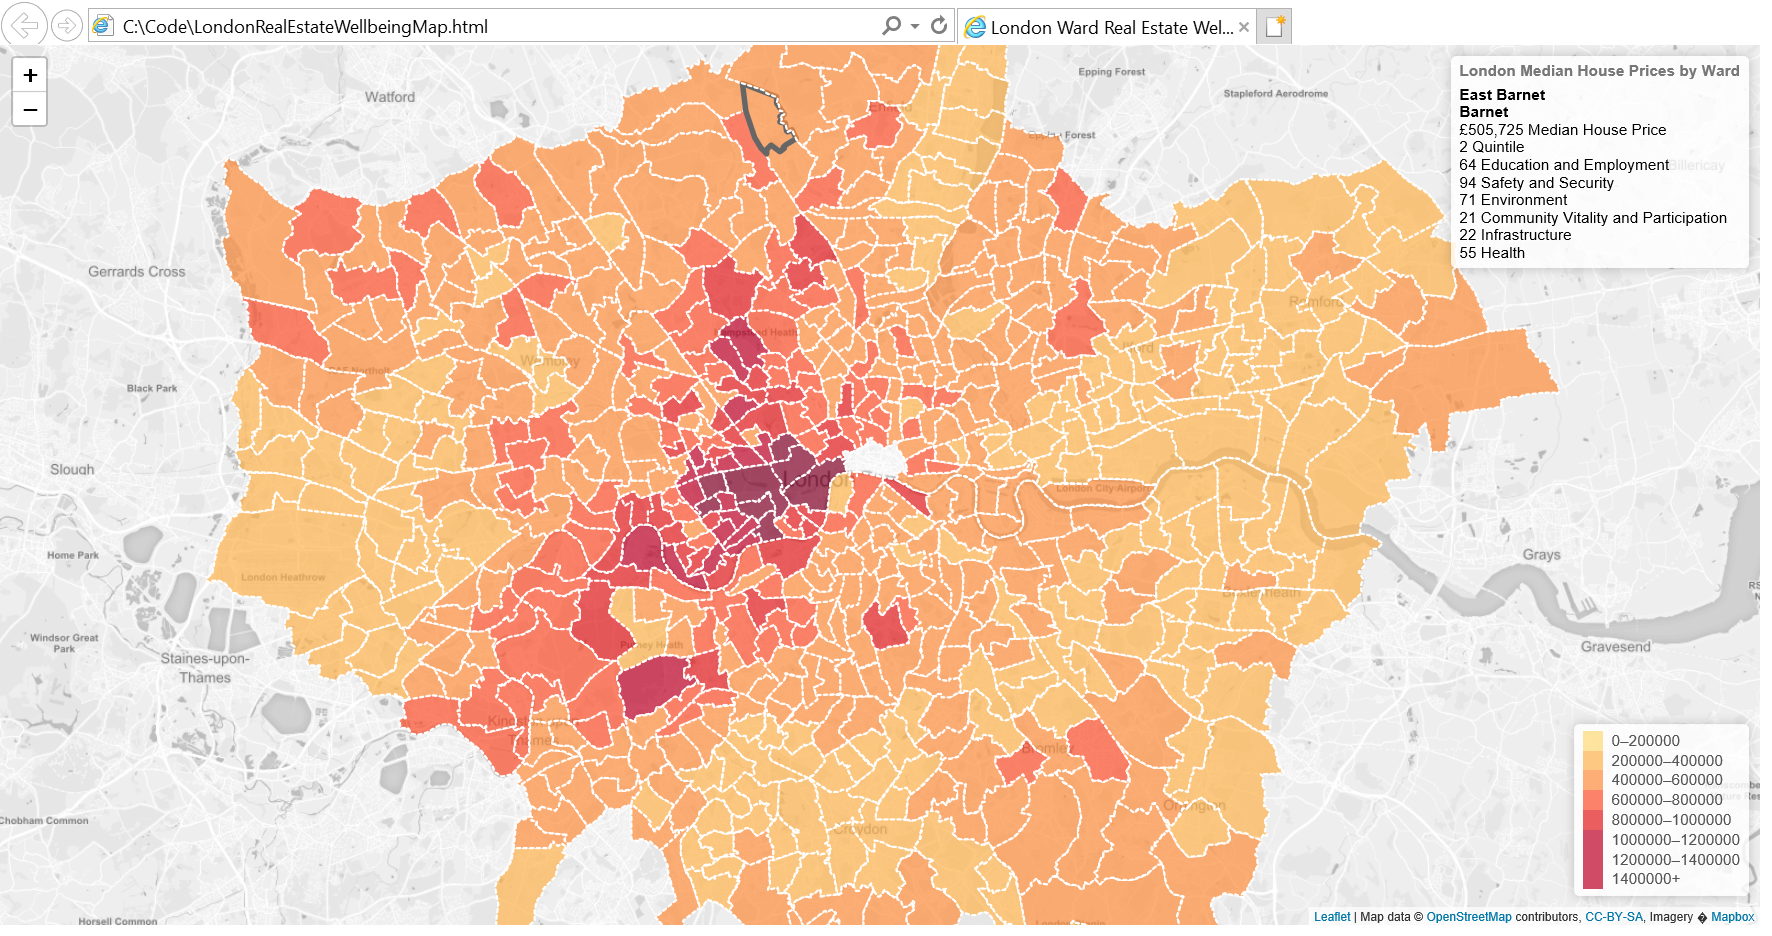
\includegraphics[scale=0.3]{figures/trailer_1}
\decoRule
\caption{Visualisation of median house prices by ward in London. Hovering over a particular ward will provide information on the well-being indices for that ward and the modelled median house prices and associated quintiles.}
\end{figure}
